\documentclass[10pt, compress, handout]{beamer} % no animations
%\documentclass[10pt, compress]{beamer}
\usetheme{m}

\usepackage{booktabs}
\usepackage[scale=2]{ccicons}
\usepackage{minted}
\usepackage{color}
\usepackage{subfig}
\usepackage{xltxtra}
\usepackage{xgreek}	
\usepackage{amsfonts}
\usepackage[Greek,Latin]{ucharclasses}
\setTransitionsForGreek{\setlanguage{greek}}{\setlanguage{american}}
\setmainfont[Kerning=On,Mapping=tex-text]{Linux Libertine O}
\usepackage{amsmath}
\usepackage{amssymb}
\usepackage{outlines}
\usepackage[normalem]{ulem}
\usepackage{url}
\usepackage{tabularx}

\usepackage{placeins}

\usepackage{multirow}

\usemintedstyle{trac}

\usepackage[backend=biber, sorting=none, maxcitenames=2]{biblatex}
\addbibresource{references.bib} % The filename of the bibliography

\title{Ανάπτυξη Ρομποτικού Οχήματος Εδάφους με Κινηματικό Μοντέλο 4WS4WD και Υλοποίηση Συστήματος για Αυτόνομη Εξερεύνηση σε Άγνωστο Περιβάλλον}
\date{\today}
\author{Γεώργιος Κούρος}
\institute{Αριστοτέλειο Πανεπιστήμιο Θεσσαλονίκης\\[-0.1cm]Τμήμα Ηλεκτρολόγων Μηχανικών και Μηχανικών Υπολογιστών\\[-0.1cm]Τομέας Ηλεκτρονικής και Υπολογιστών}


\begin{document}

\maketitle

%%%%%%%%%%%%%%%%%%%%%%%%%%%%%%%%%%%%%%%%%%%%%%%%%%%%%%%%%%%%%%%%%%%%%%%%%%%%%%%%%%%%%%%%%%%%%%
\begin{frame}[fragile]
\frametitle{Κίνητρο}
\begin{figure}[!ht] \centering
\begin{tikzpicture}
  \node (pandora_tracked_robot) {\frame{\includegraphics[height=4.5cm]{pandora_tracked_robot.png}}};
  \pause
  \node (pandora_skid_steer_robot) at (pandora_tracked_robot.south east) [yshift=1cm] [xshift=2cm] {\frame{\includegraphics[height=5cm]{pandora_skid_steer_robot.png}}};
  \pause
  \node (pandora_monstertruck) at (pandora_skid_steer_robot.south west) [yshift=1cm] [xshift=1cm] {\frame{\includegraphics[height=5cm]{pandora_monstertruck.png}}};
\end{tikzpicture}
\end{figure}
\end{frame}

%%%%%%%%%%%%%%%%%%%%%%%%%%%%%%%%%%%%%%%%%%%%%%%%%%%%%%%%%%%%%%%%%%%%%%%%%%%%%%%%%%%%%%%%%%%%%%
%\begin{frame}[fragile]
%	\frametitle{Πρόβλημα}
%	Ανάπτυξη Αυτόνομου Ρομποτικού Οχήματος με Κινηματικό Μοντέλο 4WS4WD και Δυνατότητες Αυτόνομης Εξερεύνησης σε Άγνωστο Περιβάλλον
%	
%	\bigskip	
%	\begin{itemize}[<+- | alert@+>]
%		\item Ανάγκες σε εξοπλισμό
%		\item Δυνατότητες και περιορισμοί κίνησης
%		\item Αντίληψη
%		\item Αυτόνομη Λειτουργία
%		\item Εργαλεία προς Αξιοποίηση
%	\end{itemize}
%\end{frame}

%%%%%%%%%%%%%%%%%%%%%%%%%%%%%%%%%%%%%%%%%%%%%%%%%%%%%%%%%%%%%%%%%%%%%%%%%%%%%%%%%%%%%%%%%%%%%%
\begin{frame}[fragile]
	\frametitle{Επισκόπιση}
	\textbf{Τμήματα:}
	\begin{itemize}[<+- | alert@+>]
		\item{Ρομποτική Πλατφόρμα Monstertruck}
		\item{Κινηματική Ανάλυση}
		\item{Εκτίμηση Κατάστασης και Χαρτογράφηση}
		\item{Αυτόνομη Πλοήγηση και Εξερεύνηση}
		\item{Αρχιτεκτονική Συστήματος}
		\item{Πειράματα}
	\end{itemize}
\end{frame}

%%%%%%%%%%%%%%%%%%%%%%%%%%%%%%%%%%%%%%%%%%%%%%%%%%%%%%%%%%%%%%%%%%%%%%%%%%%%%%%%%%%%%%%%%%%%%%
%%%%%%%%%%%%%%%%%%%%%%%%%%%%%%%%%%%%%%%%%%%%%%%%%%%%%%%%%%%%%%%%%%%%%%%%%%%%%%%%%%%%%%%%%%%%%%
\section{Ρομποτική Πλατφόρμα Monstertruck}

%%%%%%%%%%%%%%%%%%%%%%%%%%%%%%%%%%%%%%%%%%%%%%%%%%%%%%%%%%%%%%%%%%%%%%%%%%%%%%%%%%%%%%%%%%%%%%
\begin{frame}{Βάση}
	Τηλεκατευθυνόμενο Όχημα \textbf{Groundpounder}, της Redcat Racing.\\[1cm]
	
	\begin{minipage}{0.55\textwidth}
		\includegraphics[width=\textwidth]{Figures/groundpounder.jpg}
	\end{minipage}
	\begin{minipage}{0.4\textwidth}
		\begin{itemize}
			\item Τετρακίνηση - 4WD
			\item Τετραδιεύθυνση - 4WS
			\item Αναρτήσεις
			\item Μεταλλικό Σασί
			\item Τροχοί Offroad
		\end{itemize}
	\end{minipage}
	
\end{frame}

%%%%%%%%%%%%%%%%%%%%%%%%%%%%%%%%%%%%%%%%%%%%%%%%%%%%%%%%%%%%%%%%%%%%%%%%%%%%%%%%%%%%%%%%%%%%%%%
%\begin{frame}{Εξοπλισμός}
%	\begin{figure}
%		\centering
%		\subfloat{{\includegraphics[width=0.4\linewidth]{Figures/servo.jpg}}} \hspace{1cm}
%		\subfloat{\frame{\includegraphics[width=0.4\linewidth]{Figures/maxon_motor.png}}}\\
%		\subfloat{{\includegraphics[width=0.4\linewidth]{Figures/dynamixel.jpg}}}
%	\end{figure}
%\end{frame}
%
%%%%%%%%%%%%%%%%%%%%%%%%%%%%%%%%%%%%%%%%%%%%%%%%%%%%%%%%%%%%%%%%%%%%%%%%%%%%%%%%%%%%%%%%%%%%%%%
%\begin{frame}{Αισθητήρες}
%	\begin{figure}
%		\centering
%		\subfloat{{\includegraphics[width=0.4\linewidth]{Figures/compass.jpg}}} \hspace{1cm}
%		\subfloat{\includegraphics[width=0.4\linewidth]{Figures/hokuyo.jpg}}\\[0.5cm]
%		\subfloat{{\includegraphics[width=0.25\linewidth]{Figures/webcam.jpg}}}
%	\end{figure}	
%\end{frame}
%
%%%%%%%%%%%%%%%%%%%%%%%%%%%%%%%%%%%%%%%%%%%%%%%%%%%%%%%%%%%%%%%%%%%%%%%%%%%%%%%%%%%%%%%%%%%%%%%
%\begin{frame}{Υπολογιστής}
%	\begin{minipage}{0.49\textwidth}
%		\centering
%		\includegraphics[width=\linewidth]{Figures/odroid-xu4.jpg}
%	\end{minipage}
%	\begin{minipage}{0.49\textwidth}
%		\centering
%		\includegraphics[width=\linewidth]{Figures/odroid_specs.png}
%	\end{minipage}
%\end{frame}


%%%%%%%%%%%%%%%%%%%%%%%%%%%%%%%%%%%%%%%%%%%%%%%%%%%%%%%%%%%%%%%%%%%%%%%%%%%%%%%%%%%%%%%%%%%%%%
\begin{frame}{Εξοπλισμός}
	\begin{figure}
		\includegraphics[width=\linewidth]{Figures/electronics.png}
	\end{figure}
\end{frame}

%%%%%%%%%%%%%%%%%%%%%%%%%%%%%%%%%%%%%%%%%%%%%%%%%%%%%%%%%%%%%%%%%%%%%%%%%%%%%%%%%%%%%%%%%%%%%%
\begin{frame}{Τελική Ρομποτική Πλατφόρμα}
	\begin{center}
		\frame{\includegraphics[width=0.8\linewidth]{Figures/pandora_monstertruck.png}}
	\end{center}
\end{frame}

%%%%%%%%%%%%%%%%%%%%%%%%%%%%%%%%%%%%%%%%%%%%%%%%%%%%%%%%%%%%%%%%%%%%%%%%%%%%%%%%%%%%%%%%%%%%%%
%%%%%%%%%%%%%%%%%%%%%%%%%%%%%%%%%%%%%%%%%%%%%%%%%%%%%%%%%%%%%%%%%%%%%%%%%%%%%%%%%%%%%%%%%%%%%%
\section{Κινηματική Ανάλυση}

%%%%%%%%%%%%%%%%%%%%%%%%%%%%%%%%%%%%%%%%%%%%%%%%%%%%%%%%%%%%%%%%%%%%%%%%%%%%%%%%%%%%%%%%%%%%%%
\begin{frame}{Σύστημα Τετρακίνησης}
	\begin{equation*}
	\omega_{wheel} = \omega_{motor} / (\lambda_{gearbox} \times \lambda_{spur\_pinion} \times \lambda_{transfer\_case} \times \lambda_{differential}) = \omega_{motor} / 644
	\end{equation*}\\[-0.3cm]
	\begin{figure}
		\centering
		\subfloat{{
\includegraphics[width=0.7\linewidth]{Figures/drivetrain.png}}}\\[0.15cm]
		\subfloat{\frame{\includegraphics[height=2cm]{Figures/spur_and_pinion_gears.png}}}
		\hspace{0.5cm}
		\subfloat{\frame{\includegraphics[height=2cm]{Figures/transfer_case.png}}}
		\hspace{0.5cm}
		\subfloat{\frame{\includegraphics[height=2cm]{Figures/differential.png}}}	
	\end{figure}
\end{frame}

%%%%%%%%%%%%%%%%%%%%%%%%%%%%%%%%%%%%%%%%%%%%%%%%%%%%%%%%%%%%%%%%%%%%%%%%%%%%%%%%%%%%%%%%%%%%%%
\begin{frame}{Σύστημα Τετραδιεύθνσης}
	\begin{figure}
		\centering
		\subfloat{{\includegraphics[width=0.5\linewidth]{Figures/my_drag_link_steering.png}}} \\[0.15cm]
		\subfloat{{\includegraphics[height=4cm]{Figures/drag_link_analysis.png}}}
		\hspace{0.5cm}
		\subfloat{{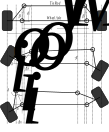
\includegraphics[height=4cm]{Figures/trapezoid_steering_mechanism}}} \\[0.05cm]
		\subfloat{{\includegraphics[width=\linewidth]{Figures/steering_transfer.png}}}
	\end{figure}
\end{frame}

%%%%%%%%%%%%%%%%%%%%%%%%%%%%%%%%%%%%%%%%%%%%%%%%%%%%%%%%%%%%%%%%%%%%%%%%%%%%%%%%%%%%%%%%%%%%%%
\begin{frame}{Κινηματικό Μοντέλο Ackermann}
	\begin{figure}
		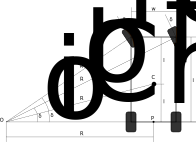
\includegraphics[height=5cm]{Figures/ackermann_model.png}
	\end{figure}
	\textbf{Συνθήκη Ackermann: }
	\begin{equation*}
		\cot{\delta_i} - \cot{\delta_o} = w / l
	\end{equation*}
\end{frame}

%%%%%%%%%%%%%%%%%%%%%%%%%%%%%%%%%%%%%%%%%%%%%%%%%%%%%%%%%%%%%%%%%%%%%%%%%%%%%%%%%%%%%%%%%%%%%%
\begin{frame}{Κινηματικό Μοντέλο Τετραδιεύθυνσης (4WS)}
	\begin{figure}[!ht]
		\subfloat{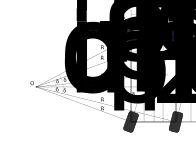
\includegraphics[height=5.2cm]{Figures/4ws_model.png}}
		\subfloat{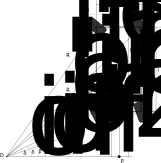
\includegraphics[height=5cm]{Figures/pos_4ws_model.png}}		
	\end{figure}
	\textbf{Συνθήκη Τετραδιεύθυνσης:}
	\begin{equation*}
		\frac{1}{\cot{\delta_{of}} - \cot{\delta_{if}}} + \frac{1}{\cot{\delta_{or}} - 	\cot{\delta_{ir}}} = \frac{l}{w}
	\end{equation*}
\end{frame}

%%%%%%%%%%%%%%%%%%%%%%%%%%%%%%%%%%%%%%%%%%%%%%%%%%%%%%%%%%%%%%%%%%%%%%%%%%%%%%%%%%%%%%%%%%%%%%
\begin{frame}{Κινηματικό Μοντέλο Ρομποτικής Πλατφόρμας Monstertruck}
	\begin{figure}
		\subfloat{\includegraphics[height=3.0cm]{Figures/steer_angles_comparison.png}}
%		\hspace{1cm}
		\subfloat{\includegraphics<1>[height=3.5cm]{Figures/monstertruck_model_parallel.png}}
		\subfloat{\includegraphics<2>[height=3.5cm]{Figures/monstertruck_slip_angle_model_parallel.png}}\\
		\subfloat{\includegraphics[height=2.0cm]{Figures/monstertruck_slip_angles.png}}
	\end{figure}
	\only<2>{\textbf{Μη Ιδανική Συνθήκη Τετραδιεύθυνσης:}	
	\begin{equation*}
		\frac{1}{\cot(\delta_{of} - \alpha_{of}) - \cot(\delta_{if} + \alpha_{if})} - \frac{1}{\cot(\delta_{or} - \alpha_{or}) - \cot(\delta_{ir} + \alpha_{ir})} = \frac{l}{w}
	\end{equation*}}
	\vspace{3cm}
\end{frame}


%%%%%%%%%%%%%%%%%%%%%%%%%%%%%%%%%%%%%%%%%%%%%%%%%%%%%%%%%%%%%%%%%%%%%%%%%%%%%%%%%%%%%%%%%%%%%%
%%%%%%%%%%%%%%%%%%%%%%%%%%%%%%%%%%%%%%%%%%%%%%%%%%%%%%%%%%%%%%%%%%%%%%%%%%%%%%%%%%%%%%%%%%%%%%
\section{Εκτίμηση Κατάστασης και Χαρτογράφηση}

%%%%%%%%%%%%%%%%%%%%%%%%%%%%%%%%%%%%%%%%%%%%%%%%%%%%%%%%%%%%%%%%%%%%%%%%%%%%%%%%%%%%%%%%%%%%%%
\begin{frame}{Κατάσταση και Χαρτογράφηση}

	\begin{itemize}
		\item 6D Κατάσταση:  $s=(x,y,z,\phi,\psi,\theta)\; \text{ή}\; (x,y,z,roll,pitch,yaw)$
    	\item	\textbf{SLAM}: \textbf{S}imultaneous \textbf{L}ocalization \textbf{A}nd \textbf{M}apping
		\item 2D αλγόριθμοι SLAM $\rightarrow$ 3D πόζα $p=(x,y,\theta)$
		\item Χάρτες Πλέγματος Κατάληψης (OGM)
		\item Χαρτογράφηση, Εκτίμηση Κατάστασης $\rightarrow$ αλληλένδετα
		\item Αξιοποίηση πληροφορίας από σαρωτές λέιζερ
		\item Σταθεροποίηση του σαρωτή λέιζερ στο επίπεδο
	\end{itemize}
	\vspace{-0.5cm}
	\begin{figure}[!ht]
		\subfloat{\frame{\includegraphics[height=3.3cm]{Figures/map_and_scan.png}}}
		\hspace{0.1cm}
		\subfloat{\frame{\includegraphics[height=3.3cm]{Figures/stabilized_laser.png}}}
	\end{figure}		
\end{frame}

%%%%%%%%%%%%%%%%%%%%%%%%%%%%%%%%%%%%%%%%%%%%%%%%%%%%%%%%%%%%%%%%%%%%%%%%%%%%%%%%%%%%%%%%%%%%%%
\begin{frame}{CRSM-SLAM}
	\textbf{CRSM}: \textbf{C}ritical \textbf{R}ays \textbf{S}can \textbf{M}atching
	
	\begin{itemize}
		\item Απαιτούμενα δεδομένα: σκαναρίσματα σαρωτή λέιζερ
		\item Αντιστοίχιση σκαναρισμάτων
		\item Εντοπισμός πόζας $\rightarrow$ μετασχηματισμός διαδοχικών σκαναρισμάτων
		\item Προεπεξεργασία σκαναρισμάτων $\rightarrow$ επιλογή κρίσιμων ακτίνων
		\item Αντιστοίχιση τρέχοντος σκαναρίσματος με ολικό χάρτη\\
		$\rightarrow$ Random Restart Hill Climbing (RRHC)
	\end{itemize}
	\begin{figure}
		\includegraphics[height=3.5cm]{Figures/crsm_slam_diagram.png}
	\end{figure}
\end{frame}

%%%%%%%%%%%%%%%%%%%%%%%%%%%%%%%%%%%%%%%%%%%%%%%%%%%%%%%%%%%%%%%%%%%%%%%%%%%%%%%%%%%%%%%%%%%%%%
\begin{frame}{Gmapping}
	\begin{outline}
		\1 Σωματίδια (particles)
		\1 Rao-Blackwellized Φίλτρα Σωματιδίων
		\1 Εκτίμηση κατάστασης μέσω συνδυασμού
			\2 Οδομετρίας και
			\2 Αντιστοίχισης σκαναρίσματων σαρωτή λέιζερ
		\1 Υψηλή εξάρτηση χαρτογράφησης από αξιόπιστη εκτίμηση κατάστασης\\[0.5cm]
		
		\1 Εκτίμηση Κατάστασης μέσω συνδυαστικής αντίληψης
		\1 EKF: Εκτεταμένα Φίλτρα Kalman
		\1 Συνδυασμός πληροφορίας από 
			\2 οδομετρία τροχών $\rightarrow$ $(x,y,\theta)$
			\2 πυξίδα $\rightarrow$ $(roll,pitch,yaw)$
			\2 \sout{οπτική οδομετρία $\rightarrow$ $(x,y,z,roll,pitch,yaw)$}
	\end{outline}
\end{frame}

%%%%%%%%%%%%%%%%%%%%%%%%%%%%%%%%%%%%%%%%%%%%%%%%%%%%%%%%%%%%%%%%%%%%%%%%%%%%%%%%%%%%%%%%%%%%%%
%%%%%%%%%%%%%%%%%%%%%%%%%%%%%%%%%%%%%%%%%%%%%%%%%%%%%%%%%%%%%%%%%%%%%%%%%%%%%%%%%%%%%%%%%%%%%%
\section{Αυτόνομη Πλοήγηση και Εξερεύνηση}

%%%%%%%%%%%%%%%%%%%%%%%%%%%%%%%%%%%%%%%%%%%%%%%%%%%%%%%%%%%%%%%%%%%%%%%%%%%%%%%%%%%%%%%%%%%%%%
\begin{frame}{Αυτόνομη Πλοήγηση}
	\begin{itemize}
		\item Στόχος: Μετάβαση από μία αρχική πόζα $p_{init}$ σε μία τελική $p_{final}$
		\item	Αναζήτηση λύσης σε Χάρτες Κόστους\\ $\rightarrow$ αναπαράσταση ρομπότ ως  σημείο
		\item Διάσπαση Προβλήματος $\rightarrow$ Ολικό και Τοπικό πρόβλημα
		\item Κινηματικοί περιορισμοί $\rightarrow$ μεγαλύτερη πολυπλοκότητα
	\end{itemize}
	\vspace{-0.5cm}
	\begin{figure}
		\centering
		\subfloat{\includegraphics[width=0.65\linewidth]{Figures/inflated_obstacles.png}}\\[0.5cm]
		\subfloat{\includegraphics[width=0.65\linewidth]{Figures/costmaps.png}}
	\end{figure}
\end{frame}

%%%%%%%%%%%%%%%%%%%%%%%%%%%%%%%%%%%%%%%%%%%%%%%%%%%%%%%%%%%%%%%%%%%%%%%%%%%%%%%%%%%%%%%%%%%%%%
\begin{frame}{Προτάσεις}
	\begin{enumerate}
		\item Αυτόνομη Πλοήγηση με Δυναμική Παραμόρφωση Μονοπατιού (DPM)
		\vspace{-0.5cm}
		\begin{enumerate}
			\item Κατασκευή στατικού ολικού μονοπατιού $\rightarrow$ Dijkstra / A*
			\item Παραμόρφωση ολικού μονοπατιού σε τοπικό $\rightarrow$ Reeds-Shepp Band
			\item Διάσχιση τοπικού μονοπατιού με ελεγκτή ασαφούς λογικής
		\end{enumerate}
		\item Αυτόνομη Πλοήγηση με Δυναμική Ανακατασκευή Μονοπατιού (DPR)
		\begin{enumerate}
			\item Δυναμική ανακατασκευή ολικού μονοπατιού $\rightarrow$ SBPL Lattice Planner
			\item Διάσχιση τοπικού μονοπατιού με ελεγκτή ασαφούς λογικής
		\end{enumerate}
		
	\end{enumerate}
	\begin{figure}
		\centering
		\includegraphics[width=2cm]{Figures/dpm.png}
		\hspace{2cm}
		\includegraphics[width=2cm]{Figures/dpr.png}
	\end{figure}
\end{frame}

%%%%%%%%%%%%%%%%%%%%%%%%%%%%%%%%%%%%%%%%%%%%%%%%%%%%%%%%%%%%%%%%%%%%%%%%%%%%%%%%%%%%%%%%%%%%%%
\begin{frame}{DPM (1/3): Ολικό Μονοπάτι μέσω Dijkstra ή Α*}
	\begin{itemize}
		\item Αντιμετώπιση του χάρτη κόστους ως γράφο
		\item Κατασκευή ολικού μονοπατιού μεταξύ αρχικής θέσης και στόχου
		\item Dijkstra $\rightarrow$ Breadth-First Search $\rightarrow$ $f(n)=g(n)$
		\item Α* $\rightarrow$ μεταξύ Breadth-First, Best-First Search $\rightarrow$ $f(n)=g(n)+h(n)$
		\item Dijkstra $\rightarrow$ πάντα βέλτιστη λύση, αλλά Α* $\rightarrow$ αποδοτικότερος
		\item \underline{Κινηματικά μη εφικτό μονοπάτι} για Car-Like Robots
	\end{itemize}
	\vspace{-0.2cm}
	\begin{figure}
		\captionsetup[subfigure]{labelformat=empty}
		\subfloat[Dijkstra]{\includegraphics[width=0.4\linewidth]{Figures/so_dijkstra_p4.png}}
		\hspace{1cm}
		\subfloat[A*]{\includegraphics[width=0.4\linewidth]{Figures/so_astar_p4.png}}
	\end{figure}
\end{frame}

%%%%%%%%%%%%%%%%%%%%%%%%%%%%%%%%%%%%%%%%%%%%%%%%%%%%%%%%%%%%%%%%%%%%%%%%%%%%%%%%%%%%%%%%%%%%%%
\begin{frame}{DPM (2/3): Μετατροπή Μονοπατιού σε Ελαστική Ζώνη}
	\begin{itemize}
		\item Μετατροπή σε ελαστική ζώνη $\rightarrow$ σημείο σε Φούσκα (Bubble)
		\item Φούσκα: Μέγιστο τοπικό, προσβάσιμο τμήμα γύρω από μία θέση b\\
		 $\rightarrow$ $B(b) = \left\lbrace q : ||b - q|| < \rho(b)\right\rbrace$
		\item Παραμόρφωση μέσω τεχνητών
		\begin{itemize}
			\item εσωτερικών ελκτικών δυνάμεων $\rightarrow$ τάση για ευθυγράμμιση
				\begin{align*}
					\mathbf{f}_c = k_c \cdot \left( \frac{\mathbf{b}_{i-1} - \mathbf{b}_i}{||\mathbf{b}_{i-1} - \mathbf{b}_i||} + \frac{\mathbf{b}_{i+1} - \mathbf{b}_i}{||\mathbf{b}_{i+1} - \mathbf{b}_i||}  \right)
				\end{align*}
			\item εξωτερικών απωστικών δυνάμεων $\rightarrow$ απομάκρυνση από εμπόδια
				\begin{align*}
					\mathbf{f}_r = \begin{cases}
						k_r \cdot \left(\rho_0 - \rho \frac{\partial\rho}{\partial \mathbf{b}}\right) \;\; &\rho < \rho_0\\
						0 \;\; &\rho \geq \rho_0
				 \end{cases}
			 \end{align*}
		\end{itemize}
	\end{itemize}
	
	\begin{figure}
		\includegraphics[height=2.5cm]{Figures/eband.png}
	\end{figure}
\end{frame}

%%%%%%%%%%%%%%%%%%%%%%%%%%%%%%%%%%%%%%%%%%%%%%%%%%%%%%%%%%%%%%%%%%%%%%%%%%%%%%%%%%%%%%%%%%%%%%
\begin{frame}{DPM(3/3): Μετατροπή Ελαστικής Ζώνης σε Ζώνη Reeds-Shepp}
\textbf{Μονοπάτι Reeds-Shepp}: βέλτιστο μονοπάτι για ένα αυτοκίνητο που κινείται και μπρος και πίσω
	\begin{itemize}
		\item 48 τύποι μονοπατιών Reeds-Shepp βάσει των λέξεων:\\[-0.8cm] 
			\begin{align*}
	\{C|C|C,\;CC|C,\;C|CC,\;CSC,\;CC_{\beta}|C_{\beta}C,\;	C|C_{\beta}C_{\beta}|C,\;\nonumber\\C|C_{\frac{\pi}{2}}SC,\;CSC_{\frac{\pi}{2}}|C,\;C|C_{\frac{\pi}{2}}SC_{\frac{\pi}2}|C\},\;\;\; C \in \{R,L\}
			\end{align*}

		\item Σύνδεση των σημείων της ελαστικής ζώνης με μονοπάτια Reeds-Shepp
		$\rightarrow$ \textbf{Ζώνη Reeds-Shepp}\\
		$\rightarrow$ Κινηματικά εφικτό μονοπάτι
	\end{itemize}
	\vspace{-0.5cm}
	\begin{figure}
		\captionsetup[subfigure]{labelformat=empty}
		\subfloat[Ολικό Μονοπάτι]{\frame{\includegraphics[height=2cm]{Figures/rsband_global_3.png}}} \hspace{0.1cm}
		\subfloat[Ελαστική Ζώνη]{\frame{\includegraphics[height=2cm]{Figures/rsband_eband_3.png}}} \hspace{0.1cm}
		\subfloat[Ζώνη Reeds-Shepp]{\frame{\includegraphics[height=2cm]{Figures/rsband_rsband_3.png}}}
	\end{figure}
\end{frame}

%%%%%%%%%%%%%%%%%%%%%%%%%%%%%%%%%%%%%%%%%%%%%%%%%%%%%%%%%%%%%%%%%%%%%%%%%%%%%%%%%%%%%%%%%%%%%%
\begin{frame}{DPR(1/2): SBPL Lattice Planner}
	\begin{itemize}
		\item Κατάσταση $s=(x,y,\theta,\upsilon)$
		\item Δικτύωμα Καταστάσεων\\$\rightarrow$ διακριτοποίηση χώρου καταστάσεων + συνδέσεις καταστάσεων
		\item Σύνδεση μεταξύ δύο καταστάσεων\\$\rightarrow$ κινηματικά και δυναμικά εφικτό μονοπάτι
		\item Χώρος Κινήσεων: κινηματικά εφικτές κινήσεις
		\item Μονοπάτι στο δικτύωμα $\rightarrow$ συνδυασμός εφικτών κινήσεων
		\item Κατασκευή Μονοπατιού $\rightarrow$ αναζήτηση σε γράφο $\rightarrow$ ARA* ή AD*
	\end{itemize}
	\begin{figure}
		\includegraphics[width=0.45\linewidth]{Figures/motion_primitives.png}
	\end{figure}
\end{frame}

%%%%%%%%%%%%%%%%%%%%%%%%%%%%%%%%%%%%%%%%%%%%%%%%%%%%%%%%%%%%%%%%%%%%%%%%%%%%%%%%%%%%%%%%%%%%%%
\begin{frame}{DPR(2/2): ARA* και AD*}
	ARA*: Anytime Repairing A*\\
	AD*: Anytime Dynamic A*
	
	\begin{itemize}
		\item A* σε Μεγάλο πρόβλημα $\rightarrow$ παραβίαση χρονικών περιορισμών\\$\rightarrow$  παραλλαγές του A*
		\item ARA*: αρχική μη βέλτιστη λύση και συνεχή βελτίωση
		\item $\epsilon>1$: παράγοντας διαστολής κόστους μονοπατιού
		\item $f(n) = g(n) + \epsilon \cdot h(n)$
		\item Επαναχρησιμοποίηση πληροφορίας από προηγούμενες αναζητήσεις
		\item AD*: ARA* + D*/D* Lite $\rightarrow$ προσαρμογή σε δυναμικά εμπόδια
	\end{itemize}
	\begin{figure}
		\captionsetup[subfigure]{labelformat=empty}
		\subfloat[ARA*]{\includegraphics[height=2cm]{Figures/arastar.png}}
		\hspace{0.5cm}
		\subfloat[AD*]{\includegraphics[height=2cm]{Figures/adstar.png}}
	\end{figure}
\end{frame}

%%%%%%%%%%%%%%%%%%%%%%%%%%%%%%%%%%%%%%%%%%%%%%%%%%%%%%%%%%%%%%%%%%%%%%%%%%%%%%%%%%%%%%%%%%%%%%
\begin{frame}{Ασαφής Ελεγκτής Διάσχισης Μονοπατιού(1/3)}
	\begin{figure}
		\subfloat{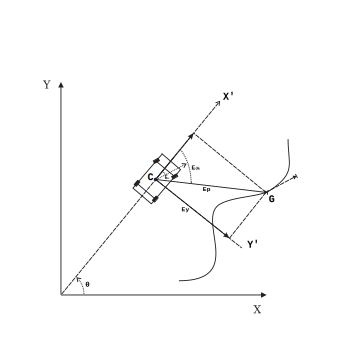
\includegraphics[height=4cm]{Figures/ptc_errors.png}}
		\hspace{1cm}
		\subfloat{\includegraphics[height=4cm]{Figures/fuzzy_ptc_inside.png}}\\[0.5cm]
		\subfloat{\includegraphics[width=0.8\linewidth]{Figures/ptc_block_diagram.png}}
	\end{figure}
\end{frame}

%%%%%%%%%%%%%%%%%%%%%%%%%%%%%%%%%%%%%%%%%%%%%%%%%%%%%%%%%%%%%%%%%%%%%%%%%%%%%%%%%%%%%%%%%%%%%%
\begin{frame}{Ασαφής Ελεγκτής Διάσχισης Μονοπατιού(2/3): Μεταβλητές}
	\begin{figure}
		\centering
		\vspace{-0.2cm}
		\subfloat{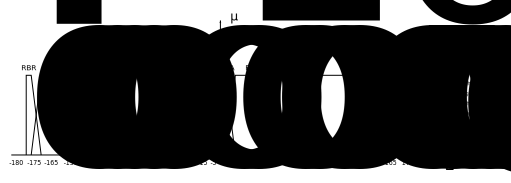
\includegraphics[height=2.7cm]{Figures/eo_ea_mf.png}}\\[-0.4cm]
		\subfloat{\includegraphics[height=2.7cm]{Figures/ep_mf.png}}
		\subfloat{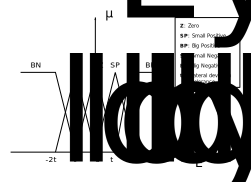
\includegraphics[height=2.7cm]{Figures/ey_mf.png}}
		\subfloat{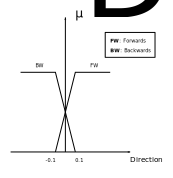
\includegraphics[height=2.7cm]{Figures/direction_mf.png}}\\[-0.4cm]
		\subfloat{\includegraphics[height=2.7cm]{Figures/speed_mf.png}}
		\subfloat{\includegraphics[height=2.7cm]{Figures/df_dr_mf.png}}
	\end{figure}
\end{frame}

\begin{frame}{Ασαφής Ελεγκτής Διάσχισης Μονοπατιού(3/3): Κανόνες}
	\begin{itemize}
		\item $\upsilon:$ ανάλογη της απόστασης $E_p$ από τον τρέχον στόχο
		\item $\delta_f:$ διόρθωση $E_\alpha$ μακρυά από τον στόχο και διόρθωση $E_o$ κοντά
		\item $\alpha_r:$ διόρθωση πλευρικής απόκλισης $E_y$ εάν $E_o$, $E_y$ μικρά
		\item Αντίστοιχη συμπεριφορά για θετική και αρνητική φορά κίνησης
	\end{itemize}
	\vspace{-0.3cm}
	\includegraphics[width=0.9\linewidth]{Figures/fuzzy_rules.png}	
\end{frame}

%%%%%%%%%%%%%%%%%%%%%%%%%%%%%%%%%%%%%%%%%%%%%%%%%%%%%%%%%%%%%%%%%%%%%%%%%%%%%%%%%%%%%%%%%%%%%%
\begin{frame}{Εξερεύνηση}
	\begin{itemize}
		\item Αυτόνομη εξερεύνηση $\rightarrow$ αυτόνομη επιλογή στόχων
		\item Κάλυψη περιβάλλοντος
		\item Μέτωπο Εξερεύνησης $\rightarrow$ σύνορο
		\item Συνάρτηση κόστους
		\item Κριτήρια επιλογής
		\begin{itemize}
			\item Μέγεθος μετώπου
			\item Μήκος μονοπατιού
			\item Γωνιακή απόκλιση
			\item Συχνότητα επιλογής
		\end{itemize}			
	\end{itemize}
\end{frame}

%%%%%%%%%%%%%%%%%%%%%%%%%%%%%%%%%%%%%%%%%%%%%%%%%%%%%%%%%%%%%%%%%%%%%%%%%%%%%%%%%%%%%%%%%%%%%%
%%%%%%%%%%%%%%%%%%%%%%%%%%%%%%%%%%%%%%%%%%%%%%%%%%%%%%%%%%%%%%%%%%%%%%%%%%%%%%%%%%%%%%%%%%%%%%
\section{Αρχιτεκτονική Συστήματος}

%%%%%%%%%%%%%%%%%%%%%%%%%%%%%%%%%%%%%%%%%%%%%%%%%%%%%%%%%%%%%%%%%%%%%%%%%%%%%%%%%%%%%%%%%%%%%%
\begin{frame}{ROS}
	\begin{figure}
		\includegraphics[width=0.4\linewidth]{Figures/ros.png}
	\end{figure}
	\textbf{ROS}: \textbf{R}obotic \textbf{O}perating \textbf{S}ystem
	\begin{itemize}
		\item Peer-to-Peer
			\begin{itemize}
				\item Κόμβοι $\rightarrow$ διεργασίες με δυνατότητες επικοινωνίας
				\item Επικοινωνία $\rightarrow$ messages, services, actions
			\end{itemize}
		\item Multilingual
			\begin{itemize}
				\item C++
				\item Python
			\end{itemize}
		\item Tools-Based
		\item Open Source
	\end{itemize}
\end{frame}

%%%%%%%%%%%%%%%%%%%%%%%%%%%%%%%%%%%%%%%%%%%%%%%%%%%%%%%%%%%%%%%%%%%%%%%%%%%%%%%%%%%%%%%%%%%%%%
\begin{frame}{Διάγραμμα Τμημάτων Λογισμικού}
	\begin{figure}
		\includegraphics[width=\linewidth]{component_diagram.png}
	\end{figure}
\end{frame}

%%%%%%%%%%%%%%%%%%%%%%%%%%%%%%%%%%%%%%%%%%%%%%%%%%%%%%%%%%%%%%%%%%%%%%%%%%%%%%%%%%%%%%%%%%%%%%
\begin{frame}{Προσομοίωση}	
	\begin{figure}
%		\vspace{-1cm}
		\begin{tikzpicture}
	   		\node (stdr_simulator) {{\includegraphics[height=4cm]{stdr_simulator.png}}};
		   \pause
		   \node (gazebo_simulator) at (stdr_simulator.south) [yshift=-1.25cm] [xshift=0cm] {{\includegraphics[height=4cm]{gazebo_simulator.png}}};
		\end{tikzpicture}
	\end{figure}
\end{frame}

%%%%%%%%%%%%%%%%%%%%%%%%%%%%%%%%%%%%%%%%%%%%%%%%%%%%%%%%%%%%%%%%%%%%%%%%%%%%%%%%%%%%%%%%%%%%%%
%%%%%%%%%%%%%%%%%%%%%%%%%%%%%%%%%%%%%%%%%%%%%%%%%%%%%%%%%%%%%%%%%%%%%%%%%%%%%%%%%%%%%%%%%%%%%%
\section{Πειράματα}

\begin{frame}{Πειράματα Κινηματικού Μοντέλου}
	\visible<1-3>{	
	\begin{figure}
			\centering
			\subfloat{\frame{\includegraphics[height=2.7cm]{Figures/simple_room.png}}}
			\hspace{0.6cm}
			\subfloat{\frame{\includegraphics[height=2.7cm]{Figures/pandora_arena.png}}}
	\end{figure}}
	\vspace{-0.8cm}
	\visible<2-3>{	
	\begin{figure}
			\centering
			\subfloat{{\includegraphics[height=2.2cm]{Figures/counter_steering_experiment.png}}}
			\hspace{1.2cm}
			\subfloat{\frame{\includegraphics[height=2.2cm]{Figures/counter_steering_experiment_real.png}}}
			\hspace{0.8cm}
		\subfloat{{\includegraphics[height=2.2cm]{Figures/counter_steering_exp_plot.png}}}
	\end{figure}}
	\vspace{-0.8cm}
	\visible<3>{	
	\begin{figure}
		\centering
		\subfloat{{\includegraphics[height=2.2cm]{Figures/crab_steering_experiment.png}}}
		\hspace{1.2cm}
		\subfloat{\frame{\includegraphics[height=2.2cm]{Figures/crab_steering_experiment_real.png}}}
		\hspace{0.8cm}
		\subfloat{{\includegraphics[height=2.2cm]{Figures/crab_steering_exp_plot.png}}}
	\end{figure}	}
\end{frame}

%%%%%%%%%%%%%%%%%%%%%%%%%%%%%%%%%%%%%%%%%%%%%%%%%%%%%%%%%%%%%%%%%%%%%%%%%%%%%%%%%%%%%%%%%%%%%%
\begin{frame}{Πειράματα Χαρτογράφησης}
	\visible<1-3>{\begin{minipage}{0.3\textwidth}
		\begin{figure}
			\captionsetup[subfigure]{labelformat=empty}
			\subfloat[]{\includegraphics[height=2cm]{Figures/stdr_robocup_ground_truth.png}}\\
			\subfloat[]{\includegraphics[height=2cm]{Figures/robocup_2013_arena.png}}\\
			\subfloat[]{\frame{\includegraphics[height=2cm]{Figures/csal.jpg}}}
		\end{figure}
	\end{minipage}}
	\hspace{0.4cm}
	\visible<2-3>{
	\begin{minipage}{0.3\textwidth}
		\begin{figure}
			\captionsetup[subfigure]{labelformat=empty}
			\vspace{0.2cm}
			\subfloat[]{\includegraphics[height=2cm]{Figures/stdr_robocup_crsm.png}}\\
			\subfloat[]{\includegraphics[height=2cm]{Figures/robocup_arena_crsm_map.png}}\\
			\vspace{-0.3cm}
			\subfloat[]{\frame{\includegraphics[width=2.5cm]{Figures/csal_crsm_map.png}}}
		\end{figure}
	\end{minipage}}
	\hspace{0.2cm}
	\visible<3>{
	\begin{minipage}{0.3\textwidth}
		\begin{figure}
			\centering
			\vspace{0.2cm}
			\captionsetup[subfigure]{labelformat=empty}
			\subfloat[]{\includegraphics[height=2cm]{Figures/stdr_robocup_gmapping.png}}\\
			\subfloat[]{\includegraphics[height=2cm]{Figures/robocup_arena_gmapping_map.png}}\\
			\vspace{-0.3cm}
			\subfloat[]{\frame{\includegraphics[width=2.5cm]{Figures/csal_gmapping_map.png}}}
		\end{figure}
	\end{minipage}}
\end{frame}

%%%%%%%%%%%%%%%%%%%%%%%%%%%%%%%%%%%%%%%%%%%%%%%%%%%%%%%%%%%%%%%%%%%%%%%%%%%%%%%%%%%%%%%%%%%%%%
\begin{frame}{Πειράματα Κατασκευής Ολικού Μονοπατιού (1/2)}
	\begin{table}
      \begin{tabular}{ c c }
			Dijkstra & \raisebox{-.35\height}{\subfloat{\includegraphics[height=1.8cm]{Figures/dijkstra_exp.png}}}\\[-0.2cm]
			A* & \raisebox{-.35\height}{\subfloat{\includegraphics[height=1.8cm]{Figures/astar_exp.png}}}\\[-0.2cm]
			ARA* & \raisebox{-.35\height}{\subfloat{\includegraphics[height=1.8cm]{Figures/arastar_exp.png}}}\\[-0.2cm]
			AD* &	\raisebox{-.35\height}{\subfloat{\includegraphics[height=1.8cm]{Figures/adstar_exp.png}}}
		\end{tabular}
	\end{table}
\end{frame}

%%%%%%%%%%%%%%%%%%%%%%%%%%%%%%%%%%%%%%%%%%%%%%%%%%%%%%%%%%%%%%%%%%%%%%%%%%%%%%%%%%%%%%%%%%%%%%
\begin{frame}{Πειράματα Κατασκευής Ολικού Μονοπατιού (2/2)}
\begin{table}[!ht]
\centering
\resizebox{0.8\textwidth}{!}{  
\begin{tabular}{|l|c|cc|cc|cc|cc|}
\cline{3-10}
\multicolumn{2}{l|}{}
& \multicolumn{2}{c|}{\textbf{Dijkstra}}                                                                  & \multicolumn{2}{c|}{\textbf{A*}}                                                                        & \multicolumn{2}{c|}{\textbf{ARA*}}                                                                               & \multicolumn{2}{c|}{\textbf{AD*}}                                                           \\ \cline{3-10} 
\multicolumn{2}{l|}{\multirow{-2}{*}{}}                                                                                & \multicolumn{1}{c}{\textbf{$T[s]$}} & \multicolumn{1}{c|}{\textbf{$s[m]$}} & \multicolumn{1}{c}{\textbf{$T[s]$}} & \multicolumn{1}{c|}{\textbf{$s[m]$}} & \multicolumn{1}{c}{\textbf{$s_{init}[m]$}} & \multicolumn{1}{c|}{\textbf{$s_{final}[m]$}} & \multicolumn{1}{c}{\textbf{$s_{init}[m]$}} & {\textbf{$s_{final}[m]$}} \\ \hline
\multicolumn{1}{|c|}{} & \textbf{$p_1$} & 0.035 & 6.02 & 0.027 & 6.02 & 6.68 & 5.91 & 7.45 & 5.92 \\ %\cline{2-2}
\multicolumn{1}{|c|}{} & \textbf{$p_2$} & 0.060 & 11.78 & 0.060 & 11.78 & 13.56 & 11.554 & 12.62 & 11.25  \\ 
\multicolumn{1}{|c|}{} & \textbf{$p_3$} & 0.110 & 19.34 & 0.090 & 19.34 & 19.85 & 18.73 & 23.26 & 18.66 \\
\multicolumn{1}{|c|}{\multirow{-4}{*}{\rotatebox[origin=c]{90}{\textbf{Στόχοι}}}} & \textbf{$p_4$} & 0.110 & 17.69 & 0.110 & 17.77 & 21.36 & 17.25 & 20.42 & 17.57 \\ \hline
\end{tabular}}
\end{table}
\end{frame}

%%%%%%%%%%%%%%%%%%%%%%%%%%%%%%%%%%%%%%%%%%%%%%%%%%%%%%%%%%%%%%%%%%%%%%%%%%%%%%%%%%%%%%%%%%%%%%
\begin{frame}{Πειράματα Δυναμικής Παραμόρφωσης Μονοπατιού}
	\begin{figure}
		\includegraphics[height=8cm]{Figures/rsband_exp.png}	
	\end{figure}		
\end{frame}

%%%%%%%%%%%%%%%%%%%%%%%%%%%%%%%%%%%%%%%%%%%%%%%%%%%%%%%%%%%%%%%%%%%%%%%%%%%%%%%%%%%%%%%%%%%%%%
\begin{frame}{Πειράματα Διάσχισης Μονοπατιού(1/2)}
	\begin{figure}
		\subfloat{\includegraphics[height=5.5cm]{Figures/path_tracking_flat_exp.png}}
		\subfloat{\includegraphics[height=5.4cm]{Figures/path_tracking_exp.png}}
	\end{figure}		
\end{frame}

%%%%%%%%%%%%%%%%%%%%%%%%%%%%%%%%%%%%%%%%%%%%%%%%%%%%%%%%%%%%%%%%%%%%%%%%%%%%%%%%%%%%%%%%%%%%%%
\begin{frame}{Πειράματα Διάσχισης Μονοπατιού(2/2)}
	\begin{figure}
		\includegraphics[height=8cm]{Figures/path_tracking_slope_exp.png}
	\end{figure}		
\end{frame}

%%%%%%%%%%%%%%%%%%%%%%%%%%%%%%%%%%%%%%%%%%%%%%%%%%%%%%%%%%%%%%%%%%%%%%%%%%%%%%%%%%%%%%%%%%%%%%
\begin{frame}{Πειράματα Εξερεύνησης Πραγματικού Περιβάλλοντος}
	\begin{figure}
		\centering
		\captionsetup[subfigure]{labelformat=empty}
		\subfloat[DPM]{\frame{\includegraphics[height=4.5cm]{Figures/exploration_dpm.png}}}
		\hspace{0.05\linewidth}
		\subfloat[DPR]{\frame{\includegraphics[height=4.5cm]{Figures/exploration_dpr.png}}}
	\end{figure}	
	\bigskip

	\begin{table}[!ht]
		\centering
		\begin{tabular}{|c|c|c|}	\hline
			 & $\mathbf{T_E[s]}$ & $\mathbf{S_E[m]}$\\ \hline
			\textbf{DPM} & $486$ & $114.89$\\ \hline
			\textbf{DPR} & $698$ & $93.38$\\ \hline
		\end{tabular}
	\end{table}
\end{frame}

%%%%%%%%%%%%%%%%%%%%%%%%%%%%%%%%%%%%%%%%%%%%%%%%%%%%%%%%%%%%%%%%%%%%%%%%%%%%%%%%%%%%%%%%%%%%%%
\begin{frame}{Συμπεράσματα}
	\begin{itemize}
		\item Μικρά σφάλματα κινηματικού μοντέλου
		\item Ατέλειες χαρτογράφησης, αλλά επαρκής αναπαράσταση
		\item DPM: υψηλή συχνότητα, αλλά αστάθεια υπό περιπτώσεις
		\item DPR: ευσταθής συμπεριφορά, αλλά χαμηλή συχνότητα
		\item Διάσχιση Μονοπατιού: επιτυχής αντιστάθμιση σφαλμάτων, αλλά κίνδυνος σύγκρουσης
	\end{itemize}
\end{frame}

%%%%%%%%%%%%%%%%%%%%%%%%%%%%%%%%%%%%%%%%%%%%%%%%%%%%%%%%%%%%%%%%%%%%%%%%%%%%%%%%%%%%%%%%%%%%%%
\begin{frame}{Μελλοντικές Επεκτάσεις}
	\begin{itemize}
		\item Βελτίωση	μηχανολογικής κατασκευής
		\item Επέκταση ρομποτικής αντίληψης
		\item Ενσωμάτωση αλγορίθμων ρομποτικής όρασης
		\item Αποδοτικότερος αλγόριθμος κατασκευής μονοπατιών Reeds-Shepp
		\item Διάσχιση μονοπατιού με εντοπισμό εμποδίων
	\end{itemize}
\end{frame}

%TODO ROBOT MODEL, EXPLORATION
%%%%%%%%%%%%%%%%%%%%%%%%%%%%%%%%%%%%%%%%%%%%%%%%%%%%%%%%%%%%%%%%%%%%%%%%%%%%%%%%%%%%%%%%%%%%%%
\begin{frame}{Ερωτήσεις}
	\begin{figure}
		\includegraphics[height=6cm]{Figures/question_mark.png}
	\end{figure}
\end{frame}

%%%%%%%%%%%%%%%%%%%%%%%%%%%%%%%%%%%%%%%%%%%%%%%%%%%%%%%%%%%%%%%%%%%%%%%%%%%%%%%%%%%%%%%%%%%%%%
\begin{frame}[allowframebreaks]{Βιβλιογραφία}
	\nocite{*}
	\printbibliography
\end{frame}


\end{document}
